\documentclass{article}
\usepackage[utf8]{inputenc}
\usepackage{graphicx}
\usepackage{listings}
\usepackage{xcolor}

%New colors defined below
\definecolor{codegreen}{rgb}{0,0.6,0}
\definecolor{codegray}{rgb}{0.5,0.5,0.5}
\definecolor{codepurple}{rgb}{0.58,0,0.82}
\definecolor{backcolour}{rgb}{255,255,255}

%Code listing style named "mystyle"
\lstdefinestyle{mystyle}{
  backgroundcolor=\color{backcolour},   commentstyle=\color{codegreen},
  keywordstyle=\color{magenta},
  numberstyle=\tiny\color{codegray},
  stringstyle=\color{codepurple},
  basicstyle=\ttfamily\footnotesize,
  breakatwhitespace=false,         
  breaklines=true,                 
  captionpos=b,                    
  keepspaces=true,                 
  numbers=left,                    
  numbersep=0pt,                  
  showspaces=false,                
  showstringspaces=false,
  showtabs=false,                  
  tabsize=2
}

\lstset{style=mystyle}


\title{Klinger Project 1}
\author{Jonathan Klinger }
\date{January 2021}

\begin{document}

\begin{titlepage}
    \begin{center}
        \vspace*{1cm}
            
        \Huge
        \textbf{Jonathan Klinger}
            
        \vspace{0.5cm}
        \LARGE
        5BHIF
            
        \vspace{1.5cm}
            
        \textbf{Einfacher HTTP 1.1 Client}
            
        \vfill
            
        A short introduction to HTTP 1.1, it's requests and a simple Client written in C++
            
        \vspace{0.8cm}
            
        \Large
        Abteilung Informatik\\
        HTBLuVA Wiener Neustadt\\
        Jänner 2021
            
    \end{center}
\end{titlepage}

\tableofcontents
\pagebreak

\section{HTTP}

HTTP steht für Hyper Text Transfer Protocol. Es handelt sich um ein Client/Server Protocol das ursprünglich zum Abrufen von statischen Informationen (z.B. Browser ruft eine Website ab) gedacht war.
Das Protokoll ist in der Anwendungsschicht (Application Layer) des OSI-Modells angesiedelt. Außerdem wird auf darunterliegenden Schichten mit TCP gearbeitet, was es zuverlässig macht. \\
HTTP wurde von der Internet Engineering Task Force (IETF) und dem World Wide Web Consortium standardisiert. 

\subsection{Eigenschaften}
\subsubsection{(Relativ) Einfach}
Das Protokoll arbeitet mit einfachen Anfragen und Antworten (Requests und Responses). D.h. der Client (z.B. wieder ein Webbrowser) schickt eine Anfrage, der Informationen über die Ressource die er zugeschickt bekommen möchte an den Server, der mit einer standardisierten Antwort, die im besten Fall die Ressource enthält, antwortet. Auf die verschiedenen Arten von Request und die Arten von Response Status Codes werde ich später eingehen. 

\subsubsection{Zustandslos}
HTTP ist Zustandslos, was bedeutet, dass alle Anfragen unabhängig voneinander sind. Informationen aus vorherigen Anfragen gehen verloren. Mittels Cookies in den Header-Informationen (siehe unten) können allerdings Status-Informationen zugeordnet werden. 

\subsubsection{Nicht auf Hypertext beschränkt}
Auch wenn es ursprünglich dafür gedacht war, können immer mehr beliebige Daten versendet werden. 

\subsubsection{Verhandlung der Datenräpresentation}
Die Content Negotiation wird verwendet um eine Abstimmung der Inhalte einer Ressource auf die Möglichkeiten des Clients ermöglicht.

\subsection{HTTP 1.1}
Diese Version des Protokolls wurde 1999 im RFC2616 publiziert. Eine der größten Erweiterungen war, dass der Client den Wunsch äußern kann (per Header Eintrag, siehe unten) den Verbindungsabbau zu überspringen, um dieselbe später wieder nutzen zu können. Seitdem kann auch eine TCP Verbindung für mehrere Anfragen verwendet werden können was die Ladezeiten extrem verkürzt da diese gerade beim Verbindungsaufbau langsam sind. \\
Außerdem wurde der MIME-Typ multipart/replace hinzugefügt.


\subsection{Funktionsweise}
Wie oben schon angeschnitten, Funktioniert HTTP mittel Anfrage und Antwort. Egal ob man im Browser eine URL eingibt oder ob man selbst mittels verschiedenen Technologien Anfragen versendet läuft der Ablauf zwischen Client und Server gleich ab.\\
\begin{center}
 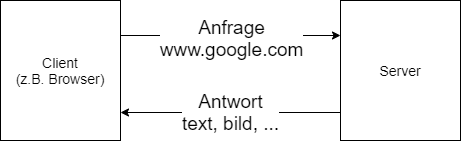
\includegraphics[scale=0.6]{funktionsweise.png}   
\end{center}

\subsubsection{Header}
Die notwendigen Informationen für eine erfolgreiche Kommunikation werden im Header hinterlegt. \\
Anfrage Header:
\begin{verbatim}
    GET /maps HTTP/1.1
    HOST: www.google.com
    Connection: close
    ...
\end{verbatim}
\\
Notwendig sind nur die 1. Beiden Zeilen. "GET" spezifiziert den Anfrage-Typ (siehe unten) danach folgt der Pfad am Server zur Ressource und die verwendete HTTP-Version. 
Die nächste Zeile spezifiziert den Host (und Portnummer) mittels URL.\\
Antwort Header:
\begin{verbatim}
    HTTP/1.1 200 OK
    Content-Type: text/html
    Date: Fri, 16 Apr 2021 00:00:00 GMT
    Server: Apache
    Set-Cookie: key=value
    ...
\end{verbatim}
\\
Der Header der Antwort ist meistens um einiges Umfangreicher als der der Anfrage. In der Ersten Zeile ist wieder die verwendete HTTP Version sowie der Status Code und die Status Message. Es folgen ein Auszug der wichtigsten Antwort-Header-Felder. \\
Der Content-Type spezifizert wie die Daten die nach dem Header folgen interpretiert werden sollten. Date enthält das Datum und die genaue Zeit wann die Antwort gesendet wurde. Das Feld Server zeigt an welche Software der Server verwendet. Und mit Set-Cookie werden die bereits erwähnten Cookies gesetzt.

\subsection{HTTP Authentifizierung}
Grundsätzlich gibt es mehrere Arten der Authentifizierung bei diesem Protokoll. Hier werde ich nur auf die Basic Authentication eingehen. Ist eine Ressource geschützt fordert der Server eine Benutzername/Passwort-Kombination an. Wird diese nicht geliefter sendet der Server einen Fehlercode (401, siehe unten). \\
Die Kombination wird im Header folgendermaßen angegeben:
\begin{verbatim}
    Authentication: Basic YmVudXR6ZXI6cGFzc3dvcnQ=
\end{verbatim}
Der hier zu sehende Text ist *nicht* verschlüsselt. Es handelt sich lediglich um die Kombination in Base64 codiert. Die Kombination muss als "benutzername:passwort" codiert werden. \\
Da es sich wie erwähnt nur um Base64 handelt ist diese Methode sehr unsicher!

\subsection{HTTP Status Codes}
Jede Anfrage wird vom Server mit einem passenden Statuscode und einer Message beantwortet. Es kann z.B. über den Erfolg oder etwaige Fehler informiert werden. \\
Hier ein Überblick über die möglichen Antworten:
\begin{itemize}
    \item 1xx - Info z.B.: 100: Continue
    \item 2xx - Erfolg z.B.: 200: OK
    \item 3xx - Umleitung z.B.: 300: Multiple Choice
    \item 4xx - Client Fehler z.B.: 401: Unauthorized
    \item 5xx - Server Fehler z.B.: 500: Internal Server Error
\end{itemize}

Mithilfe der Fehlercodes kann der Client auf verschiedene Antworten passend reagieren und gegebenfalls eine Fehlersuche erleichtern. 

\subsection{HTTP Anfragen}
\subsubsection{GET}
Ist die am meisten verwendete Methode. Es wird eine Ressource vom Server angefordert. Es besteht die Möglichkeit Argumtente im URI zu übermitteln. Laut Standard sollte mit GET nur Ressourcen abgerufen werden, sonst nichts. \\
Der Request enthält keinen Body und somit auch keine Header Elemente wie Content-size.

\subsubsection{DELETE}
Löscht die angegebene Ressource auf dem Server. Der Request enthält ebenfalls keinen Body und somit auch keine Header Elemente wie Content-size. 

\subsubsection{POST}
Schickt unbegrenzte Mengen an Daten zur weiteren Verarbeitung an den Server. Diese Daten befinden sich im Body der Nachricht. Dieser Inhalt kann einfacher Text, Key-Value-Paare oder ähnliches sein. Die Daten werden üblicherweise nicht gecached. 

\subsubsection{PUT}
Liefert die gleiche Funktionalität wie POST mit dem Unterschied, dass wenn bereits eine Ressource bereits existiert ersetzt und sonst neu erstellt wird. Der Vorgang ist somit idempotent.

\section{Das Programm}
\subsection{Aufgabenstellung}
Die Aufgabenstellung: \\

``Funktionsfähiger HTTP 1.1‐Client zum Herunterladen/Speichern von 3 
beliebigen Dateien (GET, PUT, POST, DELETE, Basisfunktionalität;
Steuerung über Kommandozeile; inkl. HTTP Basic‐Authentication,
nicht auf Header vergessen und inkl. Cookies, http‐parser kann ver‐
wendet werden)
``

\subsection{Meine Lösung}
Ich habe meine Arbeit in C++ programmiert. Es gibt einige Lösungsansätze. Für Übungszwecke habe ich mich auf die Verwendung von asio und spdlog konzentriert. 

\subsubsection{Asio}
Asio ist eine Plattform-übergreifende Bibliothek für Netzwerkprogrammierung. Die Bibliothek stellt eine Reihe an synchronen und asynchronen Funktionen
zur Verfügung. 
\\
Synchrone Kommunikation basiert auf blockierenden Operationen, während Asynchrone auf nicht blockierenden Operationen und Callbacks basiert.
\\
\\
Asio bietet die Möglichkeit mit Fehlercodes oder auch Exception die Fehler handzuhaben. 

\subsubsection{Spdlog}
Bei spdlog handelt es sich um eine header only Bibliothek die das Logging erleichtert. Die Vorteile liegen darin das es sehr schnell arbeitet und eine schöne, farbige Formatierung ermöglicht, die auch individuell angepasst werden kann.  

\subsubsection{CLI11}
Hier handelt es sich um einen Kommandozeilen-parser. Es ist wie auch spdlog eine schnelle Header-only-Bibliothek. Ein großer Vorteil ist das diese Bibliothek platformübergreifend funktioniert. Es lassen sich auch schöne Fehlermeldungen bilden. 

\subsubsection{JSON}
Die JavaScipt Object Notation ist ein Datenformat in Textform und dient zum Datenaustausch zwischen Anwendungen. Die gleichnamige Header-Only Bibliothek von dem Github-User nlohmann (siehe https://github.com/nlohmann/json) liefert die Funktionalität um diese Datenart zu lesen, interpretieren und weiter zu verarbeiten.\\
In diesem Projekt wird mit der Hilfe dieser Bibliothek aus einer JSON-Datei voreingestellte Benutzernamen und Passwörter für die jeweiligen Anfragen festgelegt.

\subsubsection{Ablauf}
Das Programm kann 3 Anfragen pro Aufruf durchführen. Diese werden per CLI11 aufgenommen. Jeder wert von jeder einzelnen Anfrage wird als Option im Aufruf des Programms aufgeführt. Diese Optionen werden in je in einer Variable gespeichert. Die Variablen jeder Anfrage werden wieder in einem Vector zusammengefasst der dann der Funktion die die eigentliche Anfrage sendet übergeben werden. 

\begin{lstlisting}[language=C++]
//Interface
CLI::App app{"Einfacher HTTP1.1 Client"};

//Erster Request
string type1 = "";
string url1  = "";
string port1 = "80";
string path1 = "/";
string file1 = "test.txt";
string user1 = "";
string pw1   = "";
string cookies1 = "";
string content_type1 = "";
string content1 = "";

//Standardauthentifizierung aus json
user1 = j["user1"];
pw1 = j["pw1"];

app.add_option("--type1", type1, "Typ von Request 1");
app.add_option("--url1",  url1,  "URL von Request 1");
app.add_option("--port1", port1, "Port von Request 1");
app.add_option("--path1", path1, "Path von Request 1");
app.add_option("--file1", file1, "Dateiname von Request 1");
app.add_option("--user1", user1, "User von Request 1");
app.add_option("--pw1",   pw1,   "Password von Request 1");
app.add_option("--cookies1", cookies1, "Cookies von Request 1");
app.add_option("--contentType1", content_type1, "Content Type von Request 1");
app.add_option("--content1", content1, "Content von Request 1");

CLI11_PARSE(app, argc, argv);

vector<string> req1{type1, url1, port1, path1, cookies1, content_type1, content1, file1, user1, pw1};
\end{lstlisting}

In diesem Ausschnitt sieht man die Initialisierung der Variablen für die Erste Anfrage, sowie die Zusammenfassung in einem Vector.  Die Reihenfolge muss in diesem Fall *nicht* stimmen (siehe unten). mittels "app.add\textunderscore option()" wird die Benutzereingabe den jeweiligen Variablen zugewiesen. In den Zeilen 17 und 18 werden die Standard- Benutzer und Passwörter zugewiesen. Falls der Benutzer jedoch diese im Aufruf angeben möchte werden diese einfach ersetzt.
\\
Das Auslesen der JSON datei funktioniert folgendermaßen:
\begin{lstlisting}[language=C+]
json j;
ifstream config_file("config.json");
string line, config;
while (getline (config_file, line)) {
  config += line;
}

config_file.close();

try { 
  j = json::parse(config);
} catch (json::parse_error& ex) {
  std::cerr << "parse error at byte " << ex.byte << std::endl;
}
\end{lstlisting}
Mithilfe der C++ Standardbibliothek fstream wird der Inhalt der Datei ausgelesen. Die Funktion json::parse() übersetzt den Inhalt dann in das JSON-Format und macht es für den Programmierer zugänglich. 
\\
\\
Diese Benutzereingabe wird jetzt so gut als Möglich auf Fehler überprüft. In der main-Funktion wird sie hinsichtlich des Anfragetyps getestet.
\begin{lstlisting}[language=C++]
if (type1 == "GET" || type1 == "DELETE") {
    send_GET_DELETE(req1, "1");
  } else if (type1 == "POST" || type1 == "PUT") {
    send_POST_PUT(req1, "1");
  } else {
    spdlog::error("1. Request: Typ nicht erkannt");
  }

  if (type2 != "") {
    if (req2[0] == "GET" || req2[0] == "DELETE") {
      send_GET_DELETE(req2, "2");
    } else if (req2[0] == "POST" || req2[0] == "PUT") {
      send_POST_PUT(req2, "2");
    } else {
      spdlog::error("2. Request: Typ nicht erkannt");
    }
  }

  if (type3 != "") {
    if (req3[0] == "GET" || req3[0] == "DELETE") {
      send_GET_DELETE(req1, "3");
    } else if (req3[0] == "POST" || req3[0] == "PUT") {
      send_POST_PUT(req3, "3");
    } else {
      spdlog::error("3. Request: Typ nicht erkannt");
    }
  }
\end{lstlisting}
Es wird davon ausgegangen das zumindest eine Anfrage durchgeführt wird. Die anderen Vektoren werden geprüft ob sie gesetzt sind, da sonst der Fehler "segmentation fault (core dumped)" aufgerufen wird da versucht wird mit nicht gestztem Speicher zu arbeiten. Wird kein passender Anfragetyp erkannt, wird mit spdlog eine Fehlermedlung angezeigt. Auch wenn andere Anfragen fehlerhaft sind, werden trotzdem die anderen durchgeführt.
\\
\\
Die Restliche Eingabe wird in den Funktionen "send\textunderscore GET\textunderscore DELETE()" und "send\textunderscore POS\textunderscore PUT()" analysiert und verarbeitet.\\
Die variable
\begin{lstlisting}[language=C++]
unsigned int file_place = 4;
\end{lstlisting}
zeigt die Position an der der Dateiname steht in dem die Antwort auf eine GET Anfrage gespeichert werden soll. Bei POST erübrigt sich das, da nicht in Dateien gespeichert wird. Diese Variable ist allerdings nicht mehr notwendig, da der Dateiname jetzt einen fixen Platz hat.
\\
\\
Ursrpünglich hat dieser if/else Teil  anhand der länge der Eingabe analysiert welche weiteren Header Felder gestzt und die variable file\textunderscore place angepasst werden muss.
\begin{lstlisting}[language=C++]
if (input.size() == 8) {
    spdlog::info(n + ". Request: Cookies erkannt");
    spdlog::info(n + ". Request: HTTP Basic Authorization erkannt");

    file_place = 7;

    string auth = input[5] + ":" + input[6];
    string base_auth = base64(auth);

    req_string = req_string + 
    "Authorization: Basic " + base_auth + "\r\n"
    "Cookie: " + input[4] + "\r\n\r\n";        
} else if (input.size() == 7) {
    spdlog::info(n + ". Request: HTTP Basic Authorization erkannt");

    file_place = 6;

    string auth = input[4] + ":" + input[5];
    string base_auth = base64(auth);

    req_string = req_string + "Authorization: Basic " + base_auth + "\r\n\r\n";
} else if (input.size() == 6) {
    spdlog::info(n + ". Request: Cookie erkannt");
    file_place = 5;

    req_string = req_string + "Cookie: " + input[4] + "\r\n\r\n";
} else {
    req_string = req_string + "\r\n";
}
\end{lstlisting}
\\
Da diese Methode auf der alten Version der Benutzereingabe die auf Positionen basierte ruht, wurde mit dem Überarbeiten der Benutzereingabe auch dieser Teil aktualisiert:
\begin{lstlisting}[language=C++]
if (input[4] != "") {
  spdlog::info(n + ". Request: Cookies erkannt");

  req_string = req_string + "Cookie: " + input[4] + "\r\n";
} 
if (input[8] != "" && input[9] != "") {
  spdlog::info(n + ". Request: HTTP Basic Authorization erkannt");

  string auth = input[8] + ":" + input[9];
  string base_auth = base64(auth);

  req_string = req_string + "Authorization: Basic " + base_auth + "\r\n";
} else if ((input[8] == "" && input[9] != "") || (input[8] != "" && input[9] == "")) {
  spdlog::error(n + ". Request: Username/Passwort nicht erkannt");
}
        
req_string = req_string + "\r\n";
\end{lstlisting}
\\
Das ist ein Auszug aus der Funktion send\textunderscore GET \textunderscore DELETE(). In der verbesserten Version werden nur die einzelnen Optionen auf ihren Inhalt geprüft und dementsprechend der HTTP-Header erweitert. Wie man erkennen kann ist der Code jetzt lesbarer und kürzer. 
\\
\\
Die Hier gezeigte Funktion "base64()" kümmert sich um die oben beschriebene codierung von benutzer:passwort. 
Da es keine C++ Funktion dafür gibt und ich in keiner der zur Verfügung stehenden Bibliotheken eine passende funktion gefunden habe, habe ich auf die Linux eigene bash Funktion mithilfe eines System-calls zugegriffen. Das funktioniert folgendermaßen:
\begin{lstlisting}[language=C++]
string base64(string str) {
  string command = "printf " + str + " | base64 > base64.txt";
  system(command.c_str());

  ifstream ifs("base64.txt");
  string ret{ std::istreambuf_iterator<char>(ifs), std::istreambuf_iterator<char>() };
  ifs.close();
  return ret;
}
\end{lstlisting}
Mithilfe des Systemcalls wird der codierte text in eine Datei geschrieben die ich dann auslesen kann. Leider Funktioniert das Programm damit nur auf Linux-Betriebssystemen, was aber in diesem Fall kein Problem ist. 
\\
\\
Die Anfrage wird mithilfe von Asio folgendermaßen gesendet. Hierbei handelt es sich um die vorherige Version. 
\begin{lstlisting}[language=C++]
char reply[1000];
error_code ec;

size_t reply_length = asio::read(sock, asio::buffer(reply), ec);

//Char[] to String
string res = "";
for (unsigned int i=0; i<reply_length; i++) {
    res = res + reply[i];
}
//Only get body/status from response
string body = res.substr(res.find("\r\n\r\n") + 4);
string status = res.substr(0, res.find("\r\n"));
\end{lstlisting}
In dem character Array reply wird die Antwort des Servers gespeichert. Diese wird dann wieder in einen string umgewandelt damit man die funktion "find()" verwenden kann.
\\
\\
In der verbesserten Version wird am senden an sich nichts geändert aber Fehler werden abgefangen. Das sieht so aus:
\begin{lstlisting}[language=C++]
size_t reply_length = asio::read(sock, asio::buffer(reply), ec);
if (ec.value() != 2) {
  spdlog::error(n + ". Request: fehlgeschlagen!");
}
\end{lstlisting}
Der Value 2 steht in diesem Fall für den Erfolg der Anfrage. Alles was nicht Erfolg ist wird hiermit abgefangen und der Benutzer wird darüber mit einer Fehlermeldung informiert.
\\
\\
Mit den Variablen "status" und "body" wird dann eine Ausgabe mittels spdlog erstellt. Außerdem wird der Body (zumindest bei GET) in eine Datei geschrieben. 
\\
Die Funktion "send\textunderscore POST\textunderscore PUT()" funktioniert im grunde genau wie das gezeigte Material mit einem unterschied in den Head-Feldern und das die Antwort nicht in einer Datei gespeichert wird.
\\
\\
Auch Fehler beim schreiben des Resultats in eine Datei werden abgefangen:
\begin{lstlisting}[language=C++]
try {
  ofstream file;
  file.open(input[7]);
  file << body;
  file.close();
  spdlog::info(n + ". Request: Datei erfolgreich erstellt");
} catch (...) {
  spdlog::error(n + ". Request: Datei erstellen fehlgeschlagen!");
}
\end{lstlisting}
Falls ein Fehler auftritt wird der Benutzer wieder informiert.
\\
\\
Hier nochmal eine vereinfachte Zusammenfassung:
\begin{center}
 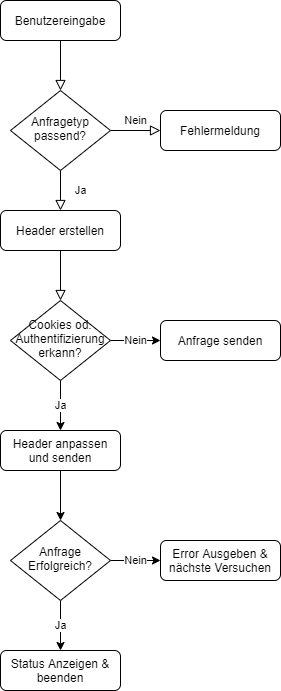
\includegraphics[scale=0.6]{ablauf.png}   
\end{center}

\subsubsection{Schwierigkeiten}
Die Lösung der Aufgabenstellung stellt den Programmierer vor einigen mehr oder weniger großen Problemen.\\
Zum einen muss man sich intensiv damit befassen für was welche Felder im HTTP-Header zuständig sind, ob sie zwingend notwendig sind und wann sie nicht gesetzt werden sollten. Z.B. habe ich anfangs aufgrund einer Fehlinterpretation das Feld "Connection" auf "keep-alive" gestellt. Das hat dazu geführt das die Ausführung des Programms sehr lange gedauert hat, da wie es der name eingtlich schon sagt die Verbindung offen gehalten wird. Das machte in diesem Fall aber keinen Sinn. 
\\
\\
Auch die Kodierung der oben genannten Benutzer/Passwort-Kombination in Base64 bietet Fehlermöglichkeiten. Anfangs habe ich den Systemaufruf mit der Funktion "echo" in die Datei geschrieben. Da kam aber ine falscher Wert raus und die Authentifizierung schlug fehl. Mit "printf" wird es allerdings richtig Kodiert und der Fehler ist behoben.
\\
\\
Auch eine Möglichkeit mein Programm zu testen war schwer zu finden. Schließlich habe ich ptsv2.com entschieden. Diese Website bietet die Möglichkeit unter selbst benannten Verzeichnissen (in meinem Fall /t/jonny) GET und POST Anfragen zu senden. Auch eine Authentifizierung kann eingestellt werden. Somit ist dieses Tool fast perfekt für meine Zwecke. Die Anfragen können eingesehen und analysiert werden bezüglich Header, Cookies und Inhalt. 

\subsubsection{Bedienung}
Für jeden zu sendenden Wert gibt es eine eigene Option. Ein Aufruf der 2 Anfragen sendet könnte so aussehen:
\begin{verbatim}
./klinger_project_2 --type1 GET --url1 ptsv2.com --path1 /t/jonny/post --port1 80 
--cookies1 cookie=value --file1 test1.txt --user1 user --pw1 password --type2 POST 
--url2 ptsv2.com --path2 /t/jonny/post --port2 80 --contentType2 text/plain 
--content2 Content ... 
\end{verbatim}
Beachte: Bei POST und PUT wird kein Dateiname erwartet! Außerdem ist als Standard-Port 80 und Standard-Path / eingestellt. Mittels der Datei config.json die sich im selben Verzeichnis befinden muss, die Benutzer/Passwort Kombinationen für alle 3 Anfragen festlegen. 
\\
\\
Eine gute Möglichkeit aufrufe zu testen ist für mich ptsv2.com. Diese Website dient als "Mülleimer" für GET und POST anfragen. Unter /t/jonny/post kann man die Anfragen senden und unter ptsv2.com/t/jonny einsehen. Diese Möglichkeit sollte nach stand 16.04.2021 noch einige Tage zur verfügung stehen. 


\section{Sources}
\begin{itemize}
  \item TCP/IP Programmierung von Prof. Kolousek
  \item HTTP-Skripten von Prof. Kolousek
  \item https://www.w3schools.com/tags/ref\textunderscore httpmethods.asps
  \item https://developer.mozilla.org/en-US/docs/Web/HTTP/Basics\textunderscore of\textunderscore HTTP/Evolution\textunderscore of\textunderscore HTTP
  \item https://www.w3.org/Protocols/rfc2616/rfc2616.html
  \item https://tools.ietf.org/html/rfc2616
\end{itemize}








\end{document}
